\documentclass[12pt]{article}
\usepackage{amsmath,amssymb,amsthm,enumerate,dsfont}
\usepackage{pdfpages}
\usepackage[a4paper,bindingoffset=0.2in,%
left=0.5in,right=0.5in,top=1in,bottom=1in,%
footskip=.25in]{geometry}

\title{Statistical Theory Homework 2}
\date{\today}
\author{Bohao Tang}

\begin{document}
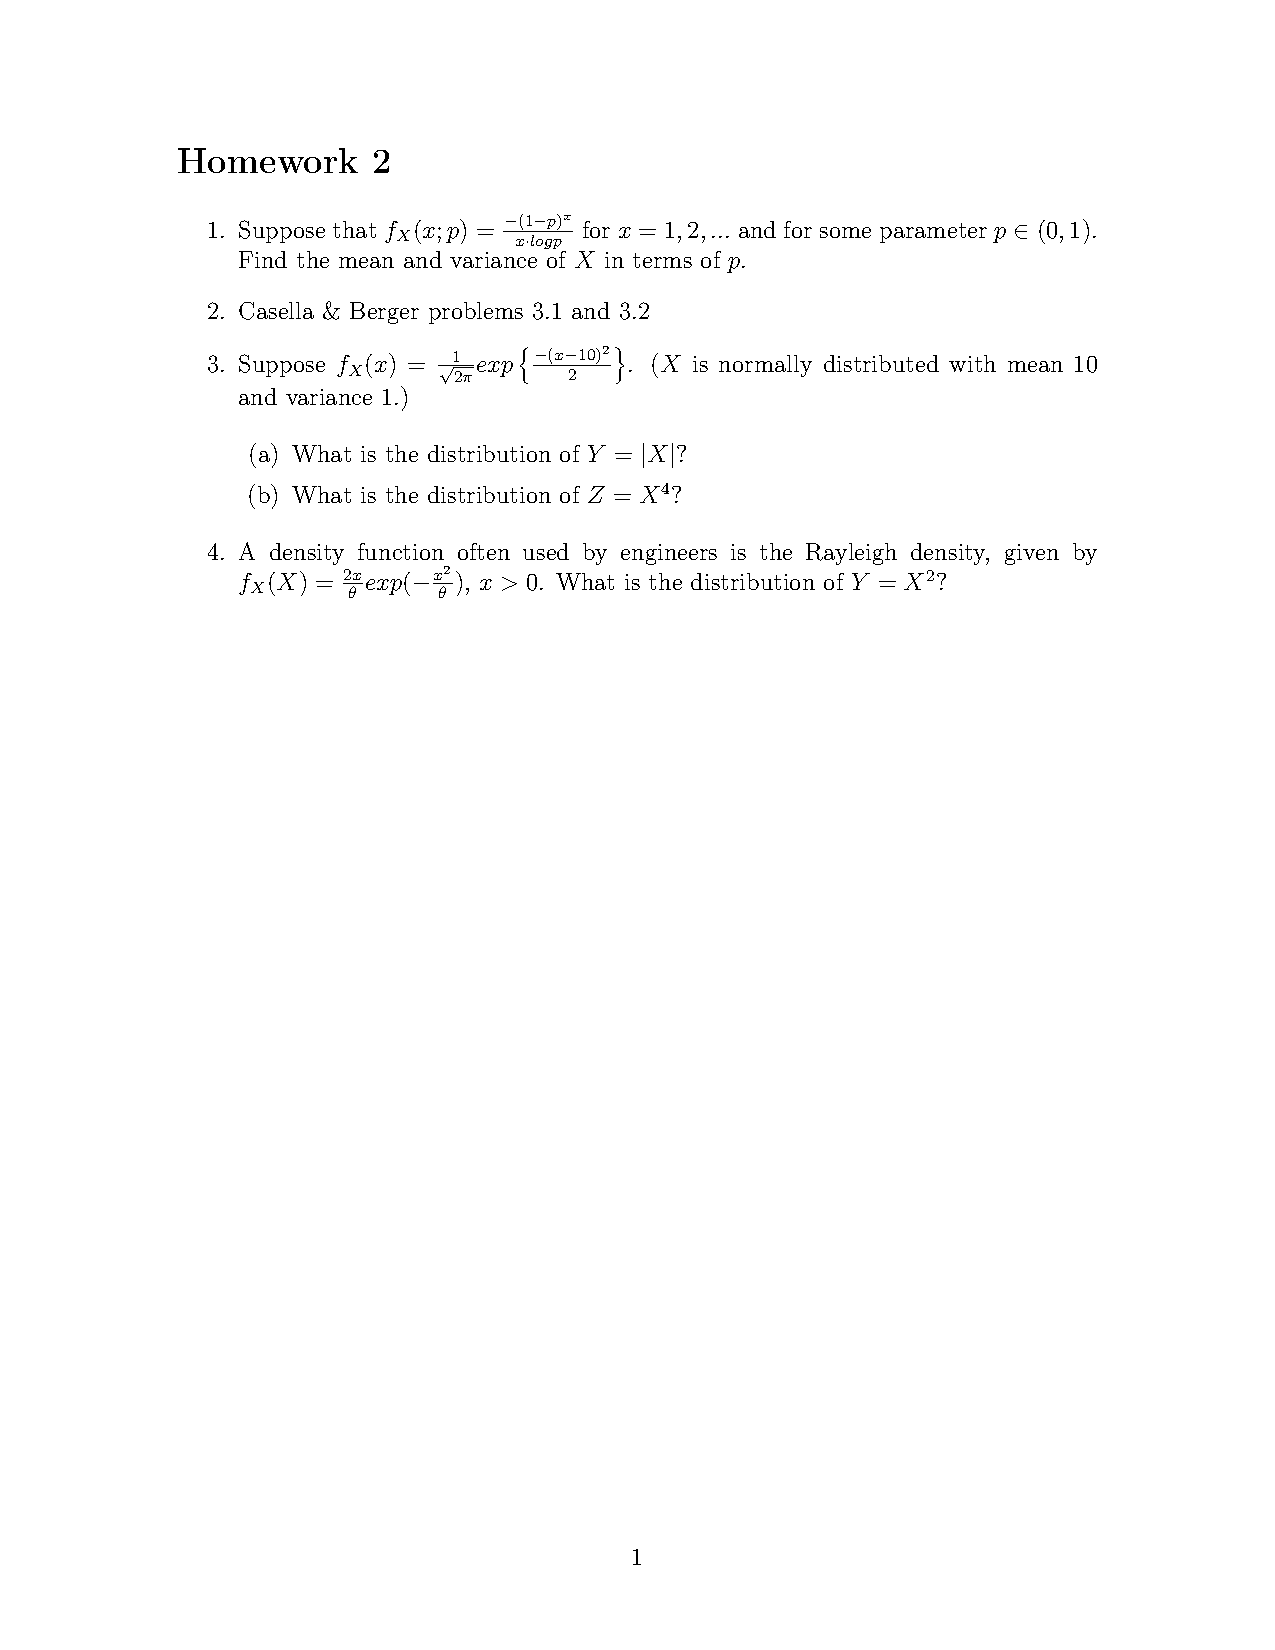
\includepdf[pages=-]{HW_2.pdf}
\maketitle

\begin{enumerate}
    \item
    First we show that $f_X(x;p)$ is a pmf. Since $\sum_{x=1}^{\infty} (1 - t)^{x-1}$ is uniformly convergent to $\frac{1}{p}$ in every subset $[p,1]$.
    We have that:
    $$\sum_{x=1}^{\infty} \frac{-(1-p)^x}{x} = \sum_x \int_1^p (1-t)^{x-1} d t= \int_1^p \sum_x (1-t)^{x-1} d t= \int_1^p \frac{1}{t} d t = \log{p}$$
    Therefore $f_X(x;p)$ is a pmf.
    Then we have:
    \begin{eqnarray}
        \mathbb{E} [X] &=& \sum_{x=1}^{\infty} x \frac{-(1-p)^x}{x \log{p}} = \frac{-(1-p) \frac{1}{1-1+p}}{\log{p}} = \frac{p-1}{p \log{p}} \\
        \mathbb{E} [X^2] &=& \sum_{x=1}^{\infty} x \frac{-(1-p)^x}{\log{p}} = \frac{1-p}{\log{p}} \frac{d }{d p} \sum_{x=1}^{\infty} (1-p)^x = \frac{p-1}{p^2\log{p}} \\
        Var[X] &=& \mathbb{E} [X^2] - \mathbb{E}^2 [X] = \frac{(1-p)(p-1-\log{p})}{p^2 \log^2{p}}
    \end{eqnarray}
    \item
    \begin{enumerate}[3.1]
        \item
        $X = N_0 - 1 + Y$, where $Y$ is uniform$(1, N_1 - N_0 + 1)$. Therefore $\mathbb{E}[X] = N_0-1+ \mathbb{E}[Y]$ and $Var[X] = Var[Y]$.
        For $Y$, we have:
        \begin{eqnarray}
            \mathbb{E}[Y] &=& \sum_{i=1}^{N_1 - N_0 + 1} \frac{i}{N_1 - N_0 + 1} = \frac{N_1 - N_0 + 2}{2} \\
            \mathbb{E}[Y^2] &=& \sum_{i=1}^{N_1 - N_0 + 1} \frac{i^2}{N_1 - N_0 + 1} = \frac{(N_1 - N_0 + 2)(2N_1 - 2N_0 + 3)}{6} \\
            Var[X] &=& Var[Y] = \mathbb{E} [Y^2] - \mathbb{E}^2 [Y] = \frac{(N_1-N_0)(N_1-N_0+2)}{12} \\
            \mathbb{E}[X] &=& \frac{N_1 - N_0 + 2}{2} + N_0 -1 = \frac{N_0+N_1}{2}        
        \end{eqnarray}
        \item
        \begin{enumerate}[(a)]
            \item
            If the lot is unacceptable, suppose there are $M$ defective parts where $M \ge 6$.
            Then the probability that the manufacturer accepts an unacceptable lot is:
            $$\textbf{P}(\text{wrong}) = \frac{\binom{100-M}{K}}{\binom{100}{K}} \le \frac{\binom{94}{K}}{\binom{100}{K}}$$
            And the '$=$' situation in '$\le$' above can be reached, so we need to let $\frac{\binom{94}{K}}{\binom{100}{K}} < 0.1$.
            Therefore $K$ should be at least $32$.
            \item
            If the lot is unacceptable, suppose there are $M$ defective parts where $M \ge 6$.
            Then the probability that the manufacturer accepts an unacceptable lot is:
            $$\textbf{P}(\text{wrong}|M) = \frac{\binom{100-M}{K}+\binom{100-M}{K-1}\binom{M}{1}}{\binom{100}{K}}$$
            Then we should choose the smallest $K$ to make $\max_{100\ge M \ge 6}\textbf{P}(\text{wrong}|M) < 0.1$.
            The numerical solution shows that $K$ need to be at least $51$.  
        \end{enumerate}
    \end{enumerate}
    \item
    We give the pdf here for $|X|$ and $X^4$.
    \begin{enumerate}[(a)]
        \item
        First, consider the cdf $F(t) = \textbf{P}(Y \le t)$, if $t < 0$, then obviously $F(t) = 0$. 
        Suppose $t \ge 0$, then $\textbf{P}(Y \le t) = \textbf{P}(-t \le X \le t) = \int_{-t}^t f_X(x) d x$. And pdf $f_Y(y) = \frac{d F(y)}{d y}$, therefore we have:
        $$f_Y(y) = (f_X(-y) + f_X(y))\mathds{1}_{y\ge 0} = \frac{\mathds{1}_{y\ge 0}}{\sqrt{2\pi}} \left(exp\{\frac{-(y+10)^2}{2}\}+exp\{\frac{-(y-10)^2}{2}\}\right)$$
        \item
        First, consider the cdf $F(z) = \textbf{P}(Z \le z)$, if $z < 0$, then obviously $F(z) = 0$. 
        Suppose $z \ge 0$, then $\textbf{P}(Y \le z) = \textbf{P}(-t^\frac{1}{4} \le X \le t^\frac{1}{4}) = \int_{-t^\frac{1}{4}}^{t^\frac{1}{4}} f_X(x) d x$. And pdf $f_Z(z) = \frac{d F(z)}{d z}$, therefore we have:
        $$f_Z(z) = \frac{t^{-\frac{3}{4}}}{4}(f_X(-z^\frac{1}{4}) + f_X(z^\frac{1}{4}))\mathds{1}_{z\ge 0} = \frac{t^{-\frac{3}{4}}\mathds{1}_{z\ge 0}}{4 \sqrt{2\pi}} \left(exp\{\frac{-(z^\frac{1}{4}+10)^2}{2}\}+exp\{\frac{-(z^\frac{1}{4}-10)^2}{2}\}\right)$$
    \end{enumerate}
    \item
    First, consider the cdf $F(y) = \textbf{P}(Y \le y)$, if $y < 0$, then obviously $F(y) = 0$. 
    Suppose $y \ge 0$, then $\textbf{P}(Y \le y) = \textbf{P}(-\sqrt{y} \le X \le \sqrt{y}) = \textbf{P}(0 < X \le \sqrt{y}) = \int_0^{\sqrt{y}} f_X(x) d x$. And pdf $f_Y(y) = \frac{d F(y)}{d y}$, therefore we have:
    $$f_Y(y) = \frac{1}{2\sqrt{y}} f_X(\sqrt{y}))\mathds{1}_{y\ge 0} = \frac{\mathds{1}_{y\ge 0}}{\theta}exp(-\frac{y}{\theta})$$
    which is a exponential distribution with mean $\theta$.
\end{enumerate}

\end{document}